\chapter{Production}
\section{Méthode de développement}
\subsection{Définition et pertinence de la méthode scrum\index{Méthode Scrum}}
Le développement du projet se fera selon la méthode Agile \key{Scrum}, comme convenu avec notre encadrant.

Cette méthode, basée sur les stratégies itératives et incrémentales, permet de produire à la fin de chaque \key{Sprint}\index{Méthode Scrum!Sprint} (incrément/itération) une version stable et testable du logiciel. Les différents événements associés à \key{Scrum} accroissent la communication grâce à des réunions quotidiennes appelées \key{mêlées}\index{Méthode Scrum!Mêlées}. Ces réunions permettent une cohésion, une coopération et une homogénéité du travail fourni par les membres de l'équipe. De plus, la présence d'artefacts c'est-à-dire d'éléments à réaliser avec des niveaux de priorité contribue à la productivité du développement.
 
Le client Antoine de \bsc{Roquemaurel} a défini le sujet et un ensemble de fonctionnalités pouvant être intégrées au logiciel. Les fonctionnalités majeures définissent les versions livrables (\key{Release}) tandis que les \key{Sprints}, propres à chaque \key{Release}, précisent les sous-fonctions à implémenter pour parvenir au résultat escompté. \\
La méthode \key{Scrum} est sujette à quelques flexibilités tel que l'ajout ou la modification de fonctionnalités durant la phase de développement afin de répondre au mieux aux besoins du client.  

\begin{figure}[H]
	\centering
	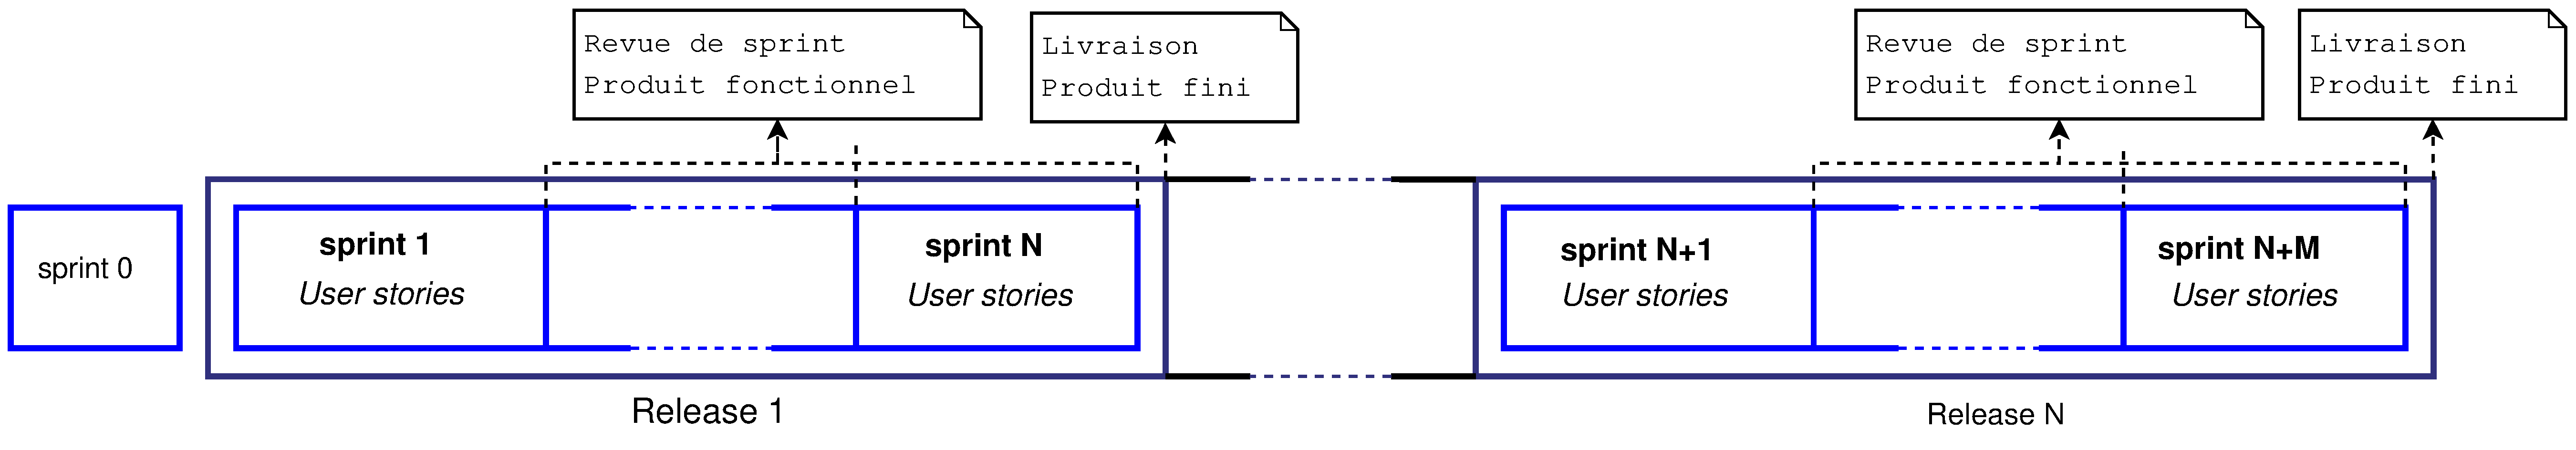
\includegraphics[width=18cm]{screens/scrum.eps}
	\caption{Fonctionnement des \key{Sprints} et \key{Releases} de la méthode \key{Scrum}}
\end{figure}

\subsection{Application de la méthode \key{Scrum} et critères de qualité}
Dans le cadre de notre projet, la durée d'un \key{Sprint} a été défini à deux semaines. Un \key{Sprint}\index{Méthode Scrum!Sprint} est constitué de \key{User Stories}\index{Méthode Scrum!User story} et de 
\key{Technicals Stories}\index{Méthode Scrum!Technical Story} qui sont préalablement définies lors de réunions quotidiennes appelées \key{mêlées}\index{Méthode Scrum!Mêlées}. Ces \key{mêlées} sont quotidiennes et organisées durant notre temps libre. En dehors de ces réunions, nous avons mis en place un salon
de discussion IRC.  

Les \key{Technical Stories} indiquent brièvement la fonction que l'on doit réaliser. Les \key{User Stories} indique les fonctionnalités du logiciel sous cette forme :

\begin{exemple}
	\textbf{En tant que} \texttt{[Personne(s) utilisant le logiciel]}\\
	\textbf{Je souhaite} \texttt{[La fonctionnalité que je désire avoir]}\\
	\textbf{Afin de} \texttt{[Objectif de la fonctionnalité]}
\end{exemple}

Chaque membre de l'équipe détermine un poids pour chaque \key{Story} c'est-à-dire une valeur indiquant sa complexité et/ou le temps nécessaire afin de la mettre en œuvre. Le poids de chaque \key{Story} est déterminé durant les \key{mêlées}\index{Méthode Scrum!Mêlées} au moyen d’un \key{Planning poker}\index{entry}.  Ainsi, chaque membre justifie le poids qu'il a déterminé et après un éventuel débat et en commun accord, une valeur est attribuée à la \key{Story}. Elle possède également des niveaux de priorité précisant
l'importance d’intégrer cette \key{Story} dans le \key{Sprint}\index{Méthode Scrum!Sprint}: 

\begin{itemize}
	\item \textit{Must} : La \key{Story} doit obligatoirement être réalisée lors du \key{Sprint}
	\item \textit{Should} : La \key{Story} devra être réalisée (dans la mesure du possible)
	\item \textit{Could} : La \key{Story} pourra être réalisée car elle n’a aucun impact sur les autres tâches
	\item \textit{Would} : La \key{Story} ne sera pas nécessairement faite et sera alors reportée au prochain \key{Sprint}
\end{itemize}

Une  \key{Story} est considérée comme terminée lorsqu'elle est fonctionnelle d’un point de vue utilisateur c'est-à-dire :
\begin{itemize}
	\item lorsque les tests unitaires (pour la base de données ou pour les modèles) sont validés
	\item lorsque les tests d’intégrations sont validés
	\item Lorsque chaque méthode est documentée
\end{itemize}

À la fin du \key{Sprint}, on présente notre logiciel à notre client, Monsieur Frédéric \bsc{Migeon} afin qu'il le valide. 
Un \key{Sprint} fournit toujours :
\begin{itemize}
	\item une démonstration des nouvelles fonctionnalités logicielles
	\item des tests unitaires
	\item une documentation du code (au format HTML et PDF)
	\item un manuel d’utilisateur à jour des nouvelles fonctionnalités
\end{itemize}

Notre projet sera réalisé en deux \key{Releases}\index{Méthode Scrum!Release} c'est-à-dire qu'il y aura deux versions livrables. Chacune de ces versions est composée de trois 
\key{Sprints}\index{Méthode Scrum!Sprint}  ayant chacun un poids moyen de 50 pour environ 10 \key{Stories}.

Les versions livrables du logiciel sont définies dans un carnet des produits (\key{Product Backlog}) qui référence l'ensemble des \key{Stories} des
différents \key{Sprints}. Ce carnet est susceptible d’évoluer en fonction des besoins du client, de nouveaux choix de conception ou encore d’éléments non prévus. 

\subsection{Organisation et rôles dans l'équipe de développement}
La méthode \key{Scrum} possède des rôles qui lui sont propres: le \key{Scrum Master}\index{Méthode Scrum!Scrum master}, le \key{Product Owner}\index{Méthode Scrum!Product Owner} et l'équipe de développement\index{Méthode Scrum!Équipe de développement}. 

\subsubsection{Scrum Master : Florent Berbie}
Le \key{Scrum Master}\index{Méthode Scrum!Scrum master} aura pour mission principale de guider les développeurs dans l'application de la méthode \key{Scrum}. Il veillera à ce que la méthode soit
comprise de tous et appliquée de façon correcte. Il aura le rôle de meneur lors de phases importantes d’application de la méthode telles que le
\key{Planning Poker} ou encore les \key{mêlées} quotidiennes.
\subsubsection{Product owner : Antoine de Roquemaurel}
Le \key{Product owner}\index{Méthode Scrum!Product owner} est la seule personne responsable du carnet de produit et de sa gestion. Ce carnet comprend l’expression de tous les items associés
à une priorité (l'importance pour le client). La compréhension de ceux-ci ainsi que la vérification du travail fourni est sous la responsabilité du
\key{Product owner}.
\subsubsection{Équipe de développement\index{Méthode Scrum!Équipe de développement} : Florent \bsc{Berbie}, Antoine de \bsc{Roquemaurel}, Cédric
\bsc{Rohaut}, Andriamihary \bsc{Razanajatovo}}
Afin d’assurer une certaine cohésion entre les membres de l’équipe, un même niveau d’implication et un travail de qualité nous avons
définis des rôles spécifiques pour chaque membre : 
\subsubsection{Directeur qualité\index{Méthode Scrum!Directeur qualité} : Cédric \bsc{Rohaut}}
Le responsable qualité sera garant de la transposition des exigences du client sous forme de solutions techniques au sein du logiciel final. De plus il devra vérifier et valider la
qualité du logiciel au travers de tests, du respect des conventions et de l'aspect général du logiciel.

\subsubsection{Directeur documentation\index{Méthode Scrum!Directeur documentation} : Andriamihary \bsc{Razanajatovo}}
Le responsable documentation sera chargé de la révision de l'ensemble des documents avant leur remise ou leur soumission aux parties prenantes
concernées. Il veillera à la qualité des aspects fondamentaux ()le fond et la forme) des documentations à fournir.

\subsubsection{Directeur technique\index{Méthode Scrum!Directeur technique} Qt, C++ : Antoine de Roquemaurel}
Le responsable technique Qt, C++ sert de support à l'équipe en cas de problèmes techniques liés au développement sur la plate-forme Qt. De par ses
connaissances acquises dans ce domaine, il sera le plus apte à aider les membres de l'équipe projet ayant des difficultés avec cette technologie.
De plus, dans le but de minimiser les couplages lors de la conception, il veillera à ce que le patron de conception MVC\footnote{Modele, Vue, Contrôleur} soit correctement utilisé. Ainsi, le code
sera clairement découpé en trois parties : modèle, vue et contrôleur ce qui permettra de s’assurer des contrôles d'interactions entre nos composants
logiciels.

\subsubsection{Autres rôles, responsabilités de chaque développeur et organisation générale}
Dans un souci d’assurance qualité, chaque responsable est en mesure de présenter les difficultés rencontrées, les différentes
solutions possibles et de justifier le choix de la technique adoptée.

Lors de la réalisation d’un cas d’utilisation (\key{issue}\index{Méthode Scrum!Issue} sur \key{Github}), celui-ci est assigné à un développeur. Une fois que ce dernier considère sa
tâche comme finie, il indique (via une \key{Pull Request}) aux autres membres de l’équipe que la tâche est soumise à la validation et à l'intégration.
Un des autres membres vérifie que la fonction est conforme à sa description, que le code est facilement compréhensible et correctement commenté. Dans
le cas ou la revue de code ne donne pleine satisfaction, le membre effectuant cette revue et les autres membres de l’équipe pourront ajouter des
commentaires pour débattre de la fonctionnalité, de l’implémentation de la fonction ou des technologies à employer. Chacun pourra
alors soumettre sa vision du problème et la manière avec laquelle il aurait résolu le problème. 

\section{Technologies utilisées}
\subsection{Architecture Logicielle}
L’objectif du logiciel est d’éditer des devis\index{FactDev!Devis} et factures\index{FactDev!Facture} et de proposer une gestion des clients\index{FactDev!Gestion des clients} : le client possède un ou plusieurs projets auxquels sont associés un ou plusieurs devis et/ou factures. 
Ainsi, l’architecture logicielle comporte une base de données de type SQLite\index{Outils!SQLite} pour la gestion des clients, de ses projets, des devis et factures associés. 
Nous utilisons un patron de conception MVC, avec un modèle qui correspond aux objets métiers Client, Projet, Factures, Devis, Prestations. Ces objets sont instanciés par les classes associées à la base de données qui réalisent ces tâches.
Enfin, nous générerons les devis et factures en LaTeX ou en PDF.

\subsection{Environnement de développement}
Le logiciel est développé à partir du \key{framework}
\footnote{Ensemble de composants logiciels structurels servant à créer les fondations d'une future application. Un framework est créé par des développeurs pour d'autres développeurs. Un framework peut être vu comme une boîte à outils.} 
Qt(version 5)\index{Outils!Qt}
en langage de programmation C++ (version 11) avec l'EDI\footnote{Environnement de Développement Logiciel} Qt Creator (version 3.3)\index{Outils!Qt Creator}. 

Les membres de l’équipe développent sur différents systèmes : MAC OS (OS X 10.10), Linux (Fedora 20 et Linux Mint 17.1). Bien que développé uniquement sur des systèmes UNIX, l’application sera compatible avec Windows. 

Afin de mener au mieux ce projet, l'équipe utilise l'outil \key{Github}, un service web d’hébergement et de gestion de développement de logiciels. 

\subsection{Outils pour la Gestion de Projet Agile}
La développement de notre logiciel s’appuie sur \key{Github}\index{Outils!Github} qui permet la gestion des différentes versions de notre logiciel. 
Cet outil est composé d’une branche directrice (appelée \key{Master}), sur laquelle se greffe de nouvelles branches : une branche par \key{Sprint}\index{Méthode Scrum!Sprint}. L’ensemble des \key{User Stories}\index{Méthode Scrum!User Story} que nous avons défini sont représentées dans \key{Github} par des \key{Issues}. Chaque \key{Issue} fait l’objet d’une nouvelle branche provenant de celle du Sprint associé. Cette gestion permet à chaque membre de développer indépendamment des autres sans entrer en conflit avec le reste l’équipe. Une fois l’issue terminée et validée par la revue de code, l’on fusionne la branche de l’issue à celle du Sprint associée afin que l’équipe bénéficie de la nouvelle version stable et fonctionnelle. On procède de la même façon en fin de \key{Sprint} en intégrant la branche de \key{Sprint} à la branche principale \key{Master}.

\begin{figure}[H]
	\centering
	\includegraphics*[width=12cm]{screens/BranchingWorkflow.eps}
	\caption{Principe du « Git Branching Workflow »}
\end{figure}

Outre la gestion des différentes versions de notre code, \key{Github} permet un suivi de notre projet. Le site internet \key{Github} dédié au projet est accessible par l’équipe et notre client Monsieur Frédéric \bsc{Migeon}. 
De plus, \key{Github} contient un Wiki avec les règles de bonne conduite et les conventions à respecter pour assurer l'homogénéité de notre projet. 

\subsection{Documentation\index{Documentation}}
La centralisation des documents se fait au moyen du Wiki\index{Documentation!Wiki} de \key{Github} et de Google Drive. 
Le Wiki de \key{Github} contient :
\begin{itemize}
	\item un tutoriel sur les méthodes de travail (Git, Scrum, C++)
	\item une convention de code à respecter (conventions de nommage des variables, des méthodes, d’organisation du code...)
	\item un tutoriel sur la documentation (\key{Doxygen})\index{Documentation!Doxygen}.
\end{itemize}

Sur Google Drive, on trouve l’ensemble des documents à rédiger en équipe. Cet outil permet notamment d’éditer un même document à plusieurs et d’être facilement accessible. Parmi les documents accessibles sur le Drive, on trouve :
\begin{itemize}
	\item le manuel de l’utilisateur\index{Documentation!Manuel de l'utilisateur}
	\item le plan d'assurance qualité\index{Documentation!Plan d'assurance qualité}
	\item le Carnet des produits \key{Product Backlog}\index{Documentation!Product Backlog}
	\item les graphiques d’avancement:\index{Graphiques d'avancement}
	\begin{itemize}
		\item Burndown chart\index{Documentation!Graphqiues d'avancement!Burndown chart}
		\item Burnup chart\index{Documentation!Graphqiues d'avancement!Burnup chart}
	\end{itemize}
	\item les Comptes rendus mensuels\index{Documentation!Comptes rendus mensuel}
	\item d’autres documents concernant le projet mais n’étant parmi ceux à rendre
\end{itemize}
 
\subsection{Assurance de la qualité du code}
Pour assurer une meilleure homogénéité, lisibilité et maintenabilité du code, nous utilisons l’outil \key{SonarQube}\index{Outils!SonarQube}, un logiciel permettant de mesurer la qualité du code source  en continu. 
Celui-ci analyse et fournit diverses informations sur le code tel que:
\begin{itemize}
	\item le pourcentage de code non documenté (ou pas assez documenté)
	\item la complexité générale du logiciel ou, au cas pas cas, des méthodes de notre programme
	\item le bon respect des conventions de codages (nommage des attributs/méthodes, indentation, …)
	\item la couverture de code (via les tests unitaires) 
	\item la duplication de code
\end{itemize}
